\documentclass[12pt]{article}
\usepackage{amsmath}
\usepackage{amsfonts}
\usepackage{amssymb}
\usepackage{amsthm}
\usepackage{graphicx}
\usepackage{float}
\usepackage{caption}
\topmargin-.5in
\textwidth6.5in
\textheight9in
\oddsidemargin0in
\evensidemargin0in

\begin{document}
\hfill {\large Project: }Bio-Physical assumptions for \textit{Myxococcus Xanthus} Polarity
\vspace{9mm}
\section*{ \centerline{August 10, 2015}
\centerline{ \bf \large report author: Francesco Pancaldi}}
The bacteria \textit{M. Xanthus} is a model organism used to study collective motions, is a Gram-negative bacteria, and is commonly found in top soil.\\
This bacteria has a capsule or rod shape, with length between 4 and 10 $\mu m$ in length and 1 $\mu m$ in diameter.\\
This bacteria uses two motility mechanisms, A-motility and S-motility. The first is mainly used to explore the environment and the second is used primarily for collective motion.\\
One of the main characteristics in \textit{M. Xanthus} movements is complete inversion in its direction of movement that happens on average every 7-9 minutes. After one of this events the bacteria moves with a preferential direction completely opposite to the one it had before.\\
These reversal events are believed to be related with the distribution of a protein called RomR inside the bacteria body.\\
Specifically this protein mostly accumulates at the poles (i.e. two extremities) of the bacteria. However, in our recent experiment we were able to visualize a significant portion of the protein diffusing in the middle of the cell (from one pole to the other).\\
The concentrations in the two poles are not identical, with the leading pole (front) having less RomR than the lagging pole (back). Moreover, a reversal in concentrations was observed in correspondence of the reversal events mentioned above.\\
Additionally during division a new concentration peak can be observed in correspondence to the division locus.\\
Also hyper reversing mutants present additional concentration spots along the cell body that seem to be fixed.\\
These empirical observations lead us to some assumptions for our 1D model in which we simulate the dynamics of the protein RomR inside the call body.\\
\begin{enumerate}
\item RomR protein exist in two forms bounded to the membrane and unbounded;
\item Each form has specific diffusion coefficient (0 or very low for the bounded one);
\item RomR can change from one form to an other depending on attachment and detachment rates;
\item RomR can bind to the membrane (i.e attach) only if free active receptors are available(i.e. not occupied or blocked);
\item Receptors are present only close to a pole or the center during division (where new poles are formed);
\item during division progressively more receptors are introduced near the center;
\item One RomR receptors can bind only a fixed amount of RomR protein;
\item RomR receptors can be either active or non-active and only active receptors can bind RomR;
\item RomR receptors are activated (or deactivated) by a protein that diffuses in the cell body and reacts with other proteins similarly to the MinCDE system in E. Coli;
\item during division the two daughter cells can exchange protein for a certain amount of time (either freely or with certain limitations);
\item When the two cells separate communication is interrupted; 
\end{enumerate}

\begin{figure}[H]
    \centering
    \includegraphics[width=0.4\textwidth]{division.jpeg}
    \caption{}
    \label{fig20}
\end{figure}

Therefore we propose the following equations for a 1D PDE model:\\ \\
Equation for RomR when not bounded to the membrane (note:$C=C(x,t)$).
\begin{equation}
\frac{\partial C}{\partial t}=\frac{\partial}{\partial x}\left(D\frac{\partial C}{\partial x}\right)- r\alpha C+R c
\end{equation}
where $D$ is the diffusion coefficient (could be space dependent), $r$ and $R$ are the binding  and unbinding rates to the RomR-receptors, and $\alpha=\min(n-c,0)$ with $n$ number of active receptors.\\ \\
Equation for RomR when bounded to the membrane (note:$c=c(x,t)$).
\begin{equation}
\frac{\partial c}{\partial t}=r\alpha C-R c 
\end{equation}
Equation for density of active receptors.
\begin{equation}
   n(x,t) = \left\{
     \begin{array}{lcr}
       f (N, k, h),& x\in [0, l_1]\cap [L-l_1, L] & t \leq T_2\\
       & &\\
 g(t)f (N, k, h) ,& x \in[L/2-l_2, L/2 +l_2 ] & T_1\leq t \leq T_2

     \end{array}
   \right.
\end{equation}
where $l_1$ and $l_2$ indicates respectively the region near the poles and near the center, $T-1$ and $T_2$ are the start and end times of division,  $N$ is the maximum density of active receptors at any given location, $f$ is a function quantifying the amount of active receptors dependent on $N$ and the quantity of chemicals $k, h$, and $g$ is a function for the growth of new receptors at the center.\\
For example
\begin{equation}
   n(x,t) = \left\{
     \begin{array}{lcr}
       N \frac{k}{k_{max}},& x\in [0, 1]\cap [9, 10] & t \leq T_2\\
       & &\\
 \frac{t-T_1}{T_2-T1}N \frac{k}{k_{max}} ,& x \in[4.5, 5.5] & T_1\leq t \leq T_2

     \end{array}
   \right.
\end{equation}
or
\begin{equation}
   n(x,t) = \left\{
     \begin{array}{lcr}
       N \left(1-\frac{k}{k_{max}}\right),& x\in [0, 1]\cap [9, 10] & t \leq T_2\\
       & &\\
 \frac{t-T_1}{T_2-T1}N \left(1-\frac{k}{k_{max}}\right) ,& x \in[4.5, 5.5] & T_1\leq t \leq T_2

     \end{array}
   \right.
\end{equation}
The variables $k, K$ are the densities for unbounded and bounded form of a chemical that interferes with the receptors and interacts with a second chemical $h,H$ as described by the following equations:
\begin{equation}
\frac{\partial K}{\partial t}=\frac{\partial}{\partial x}(D_K\frac{\partial K}{\partial x})-\frac{\sigma_1K}{1+\sigma_1'h}+\sigma_2hk
\end{equation}
\begin{equation}
\frac{\partial k}{\partial t}=\frac{\sigma_1K}{1+\sigma_1'h}-\sigma_2hk
\end{equation}
\begin{equation}
\frac{\partial H}{\partial t}=\frac{\partial}{\partial x}(D_H\frac{\partial H}{\partial x})+\frac{\sigma_4h}{1+\sigma_4'K}-\sigma_3KH
\end{equation}
\begin{equation}
\frac{\partial H}{\partial t}=-\frac{\sigma_4h}{1+\sigma_4'K}+\sigma_3KH
\end{equation}
(these equations are taken from the literature about the MinCDE system and have been shown to produce oscillation from on pole to the other with a period T dependent on the parameters).\\\\

At the moment we are dealing with the formation of the new "boundary at the center considering our diffusion coefficient to be a function of space and time close to the center of the cell.
In this way when we expand the diffusion term in our previous equation we obtain
\begin{equation}
\frac{\partial}{\partial x}\left(D\frac{\partial C}{\partial x}\right)=D\frac{\partial^2 C}{\partial x^2}+\frac{\partial D}{\partial x}\frac{\partial C}{\partial x}
\end{equation}
For $D$ a reasonable assumption will be to consider a symmetric function equal to a constant $D_0$ away from the center and with only one minimum point at the center equal to $D_0$ for $t=T_1$ and that tends to 0 when $t\rightarrow T_2$ (see figure). This way before division we have our classic diffusion term, while during division around the center we will have advective terms pointing away from the center (due to the slope of the function for $D$).

\begin{figure}[H]
    \centering
    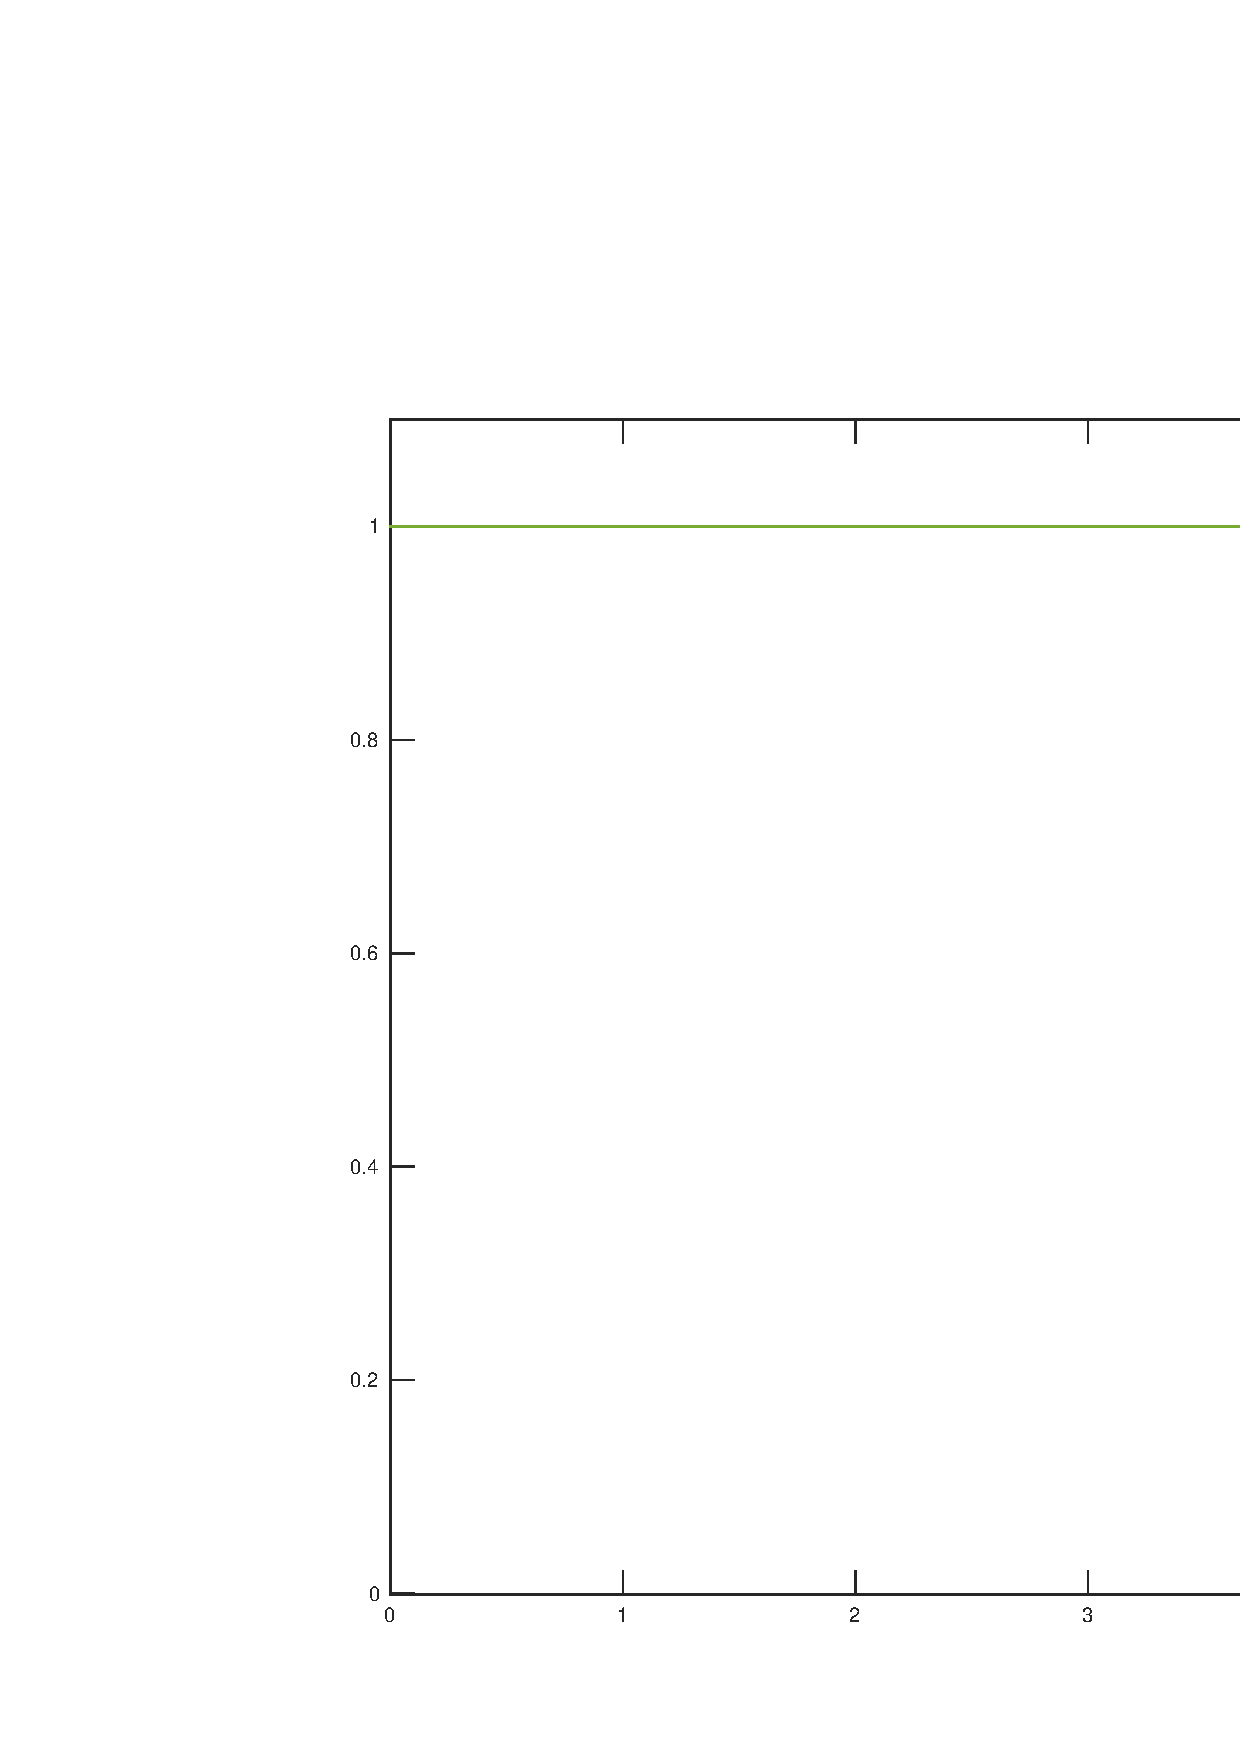
\includegraphics[width=1.2\textwidth]{diffusion.jpeg}
    \caption{Diffusion coefficient as a function of space and time. Lower minimum correspond to longer time past since division started. At the end of division the minimum is 0 (or a small $\epsilon$)}
    \label{fig20}
\end{figure}

\begin{figure}[H]
    \centering
    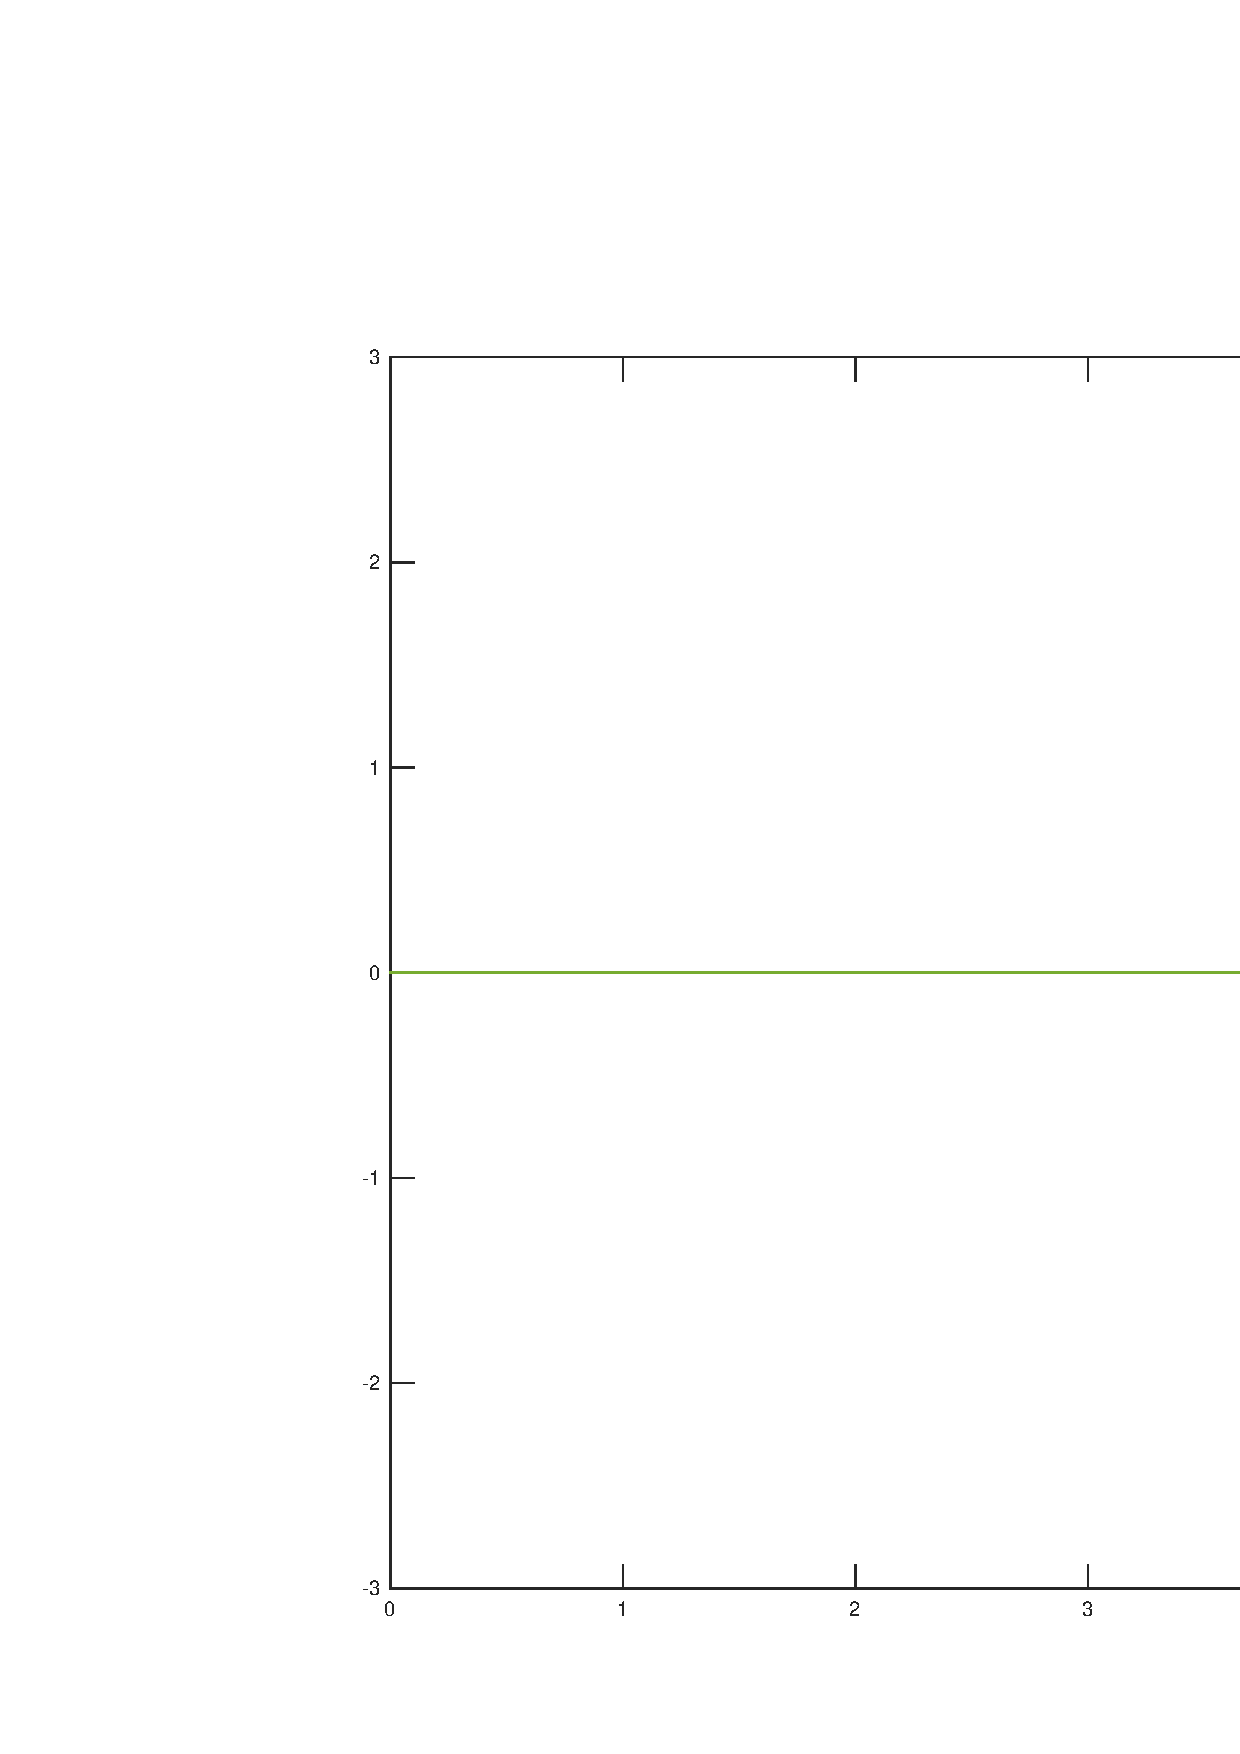
\includegraphics[width=1.2\textwidth]{advection.jpeg}
    \caption{Strength of the advective term (i.e. space derivative of $D$). Negative correspond to left direction and positive to right direction. }
    \label{fig20}
\end{figure}

Therefore, the varying diffusion coefficient acts as a repulsive "condition" at the center.\\
This choice is somewhat justifiable by the fact that the change in the domain is producing a correspondent change in the "effective" diffusibility of the RomR particles, limiting it in one of the two possible directions, due to the formation of the new boundary.\\
However, it is not clear how strong this effect should be and how fast.\\\\

Additionally, as mentioned before near the center new receptors are added (see figure) inducing some of the protein to bind to the membrane near the division site (getting stuck there). 

\begin{figure}[H]
    \centering
    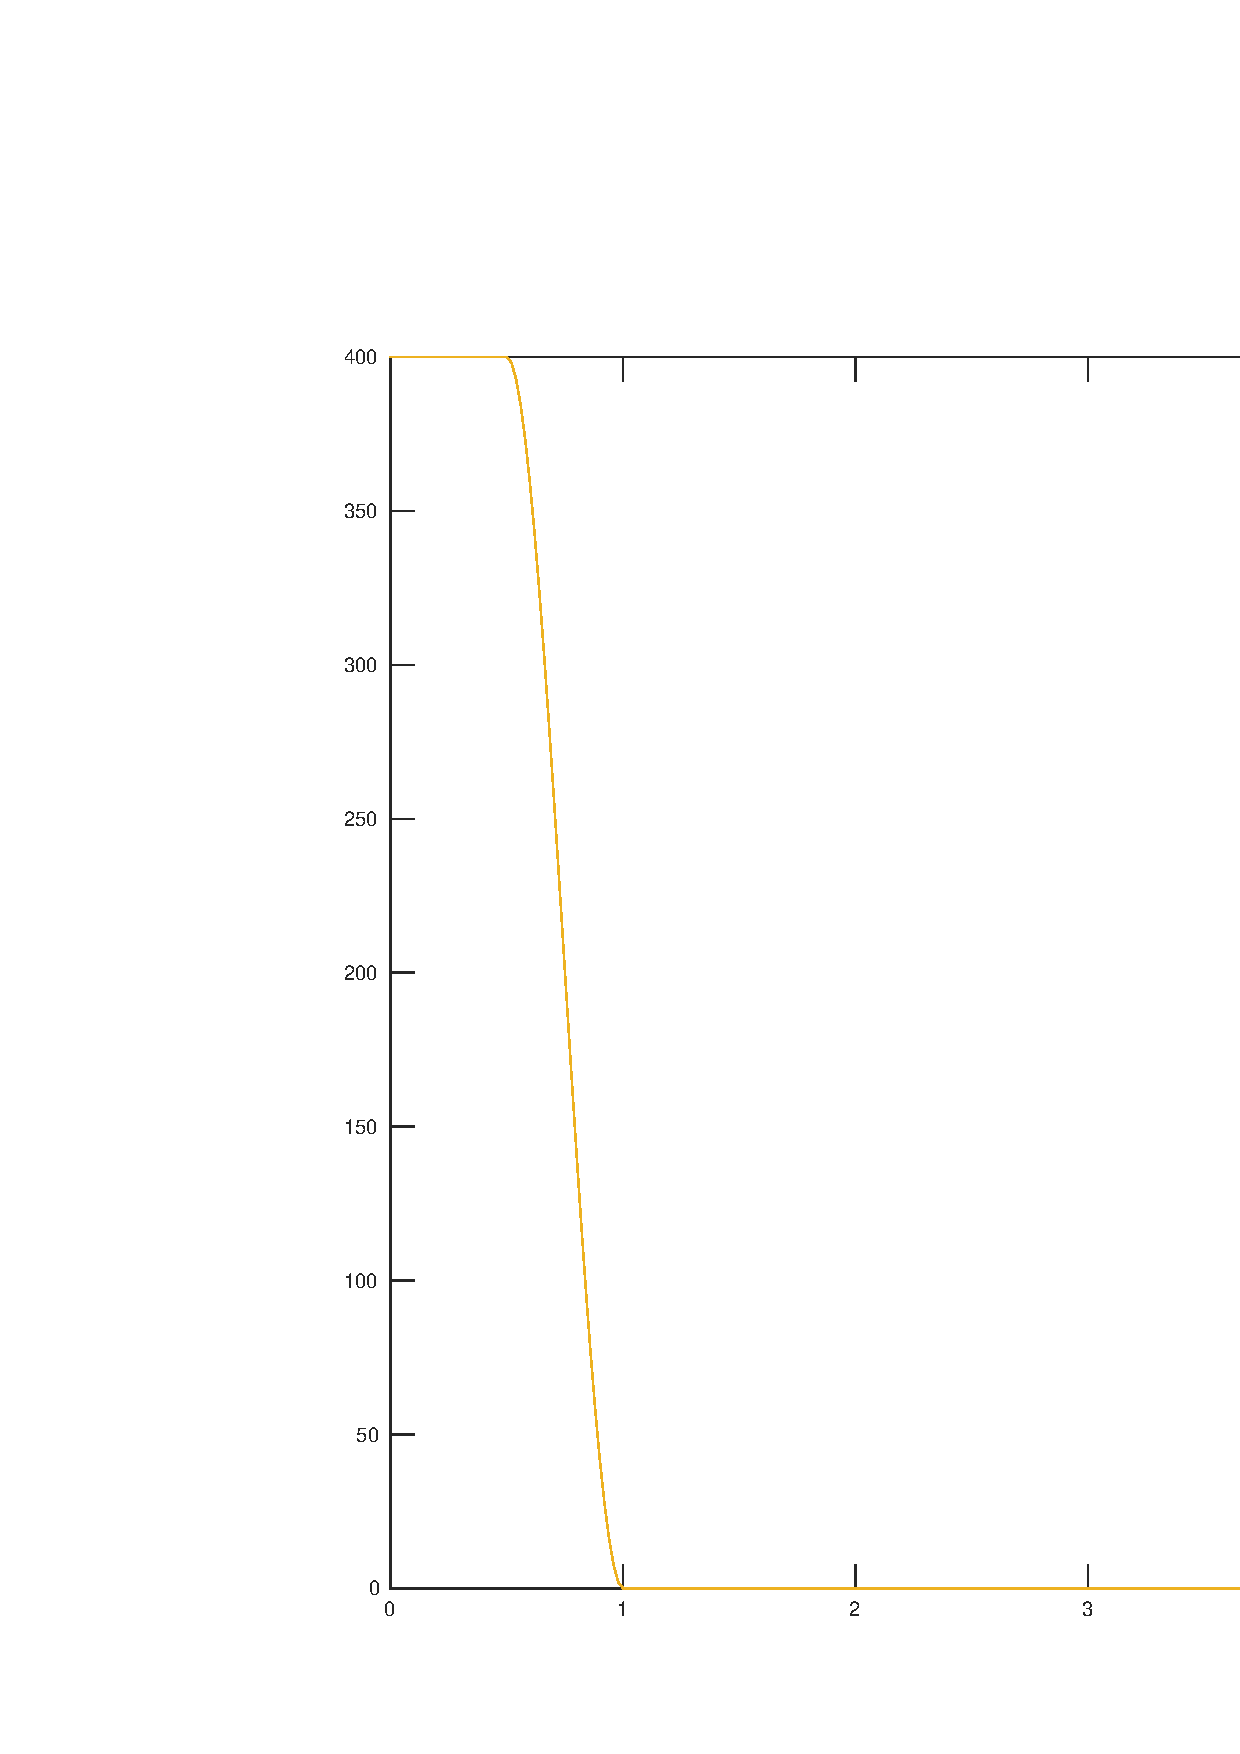
\includegraphics[width=1.2\textwidth]{receptors.jpeg}
    \caption{Number of receptors (when not affected by other chemicals) during division. Higher peak at the center correspond to more time passed since division started. }
    \label{fig20}
\end{figure}

A possible different approach to deal with the change in diffusibility near the center is to consider the conservation of mass equation as derived in sections 9.2 and 9.3 of Edelstein-Keshet book "Mathematical Models in Biology" (see link pages 393-397). The author derives a conservation equation for motion in 1D along a tube with varying cross-sectional area (in space and/or time). I am reporting the final equation here ( eq (33) in the chapter; please see the link to the chapter for more details)
\begin{equation}
\frac{\partial C(x,t)}{\partial t}=-\frac{\partial J(x,t)}{\partial x}\pm\sigma(x,t)-\frac{1}{A(x,t)}\left[J(x,t)\frac{\partial A(x,t)}{\partial x}+C(x,t)\frac{\partial A(x,t)}{\partial t}\right]
\end{equation}
where $A(x,t)$ is the cross-sectional area at time $t$ and position $x$, $J(x,t)$ is the flux, and $\sigma$ represent source/sink terms.\\\\
Then the next step to obtain a diffusion equation was to determine a relation for $J$ in terms of $C$. To do this I simply applied Fick's Law $J = -D \frac{\partial C}{\partial x} $ (with $D$ constant).
\\
Obtaining the following new equation for our $C$
\begin{equation}
\frac{\partial C(x,t)}{\partial t}= D\frac{\partial^2 C(x,t)}{\partial x^2}-\frac{1}{A(x,t)}\left[-D\frac{\partial C(x,t)}{\partial x}\frac{\partial A(x,t)}{\partial x}+C(x,t)\frac{\partial A(x,t)}{\partial t}\right]- r\alpha C+R c
\end{equation}

However, when I tried to use this in the simulation the total concentration started to grow linearly in time during division. Since we have no production this should not happen. And the conservation of mass could not be the problem, so I tried to look into the derivation of Fick's law to understand if maybe there was some assumption that was not compatible with changing cross-sectional area.\\

I proceed from a standard derivation that I believe you also use in your class.

We consider particles moving through a random walk in one dimension with length scale $\Delta x$ and time scale $\Delta t$, with $N(x, t)$ number of particles at position $x$ at time $t$.

At each given time $t$ on average half of the particles would move on the left $x-\Delta x$ and half on the right right $x+\Delta x$. Therefore the net movement to the right is:

\begin{equation}
\frac{1}{2}\left[N(x + \Delta x, t) - N(x, t)\right]
\end{equation}

Since the flux, J, is this net movement of particles across some area element "A", normal to the random walk during the interval of time $\Delta t$ we can now write:

\begin{equation}
J = - \frac{1}{2} \left[\frac{ N(x + \Delta x, t)}{A \Delta t} - \frac{ N(x, t)}{A \Delta t}\right]
\end{equation} 
Multiplying  by $(\Delta x)^2$ we get:


\begin{equation}
 J = -\frac{\left(\Delta x\right)^2}{2 \Delta t}\left[\frac{N(x + \Delta x, t)}{A (\Delta x)^2} - \frac{N(x, t)}{A (\Delta x)^2}\right]
 \end{equation}

Now we note that concentration is defined as particles per unit volume $V=A\Delta x$ giving us $C (x, t) = \frac{N(x, t)}{A \Delta x}=\frac{N(x, t)}{V}$.

Now setting $D=\frac{\left(\Delta x\right)^2}{2 \Delta t}$ our equation becomes:

\begin{equation}
 J = -D \left[\frac{C (x + \Delta x, t)}{\Delta x} - \frac{C (x , t)}{\Delta x}\right]
 \end{equation}

And in the limit for $\Delta x\rightarrow 0$ 

\begin{equation}
 J = - D \frac{\partial C}{\partial x}  
 \end{equation}
 
 When I re-considering this proof for our case however I am not sure if the passage between eqn. (15) and (16), in which the diffusion coefficient is introduced as a constant and the area is absorbed into the concentration when taking the limits, can be done as described here, since in our case $A$ depends on $x$ and $t$ and therefore as two different values at $x$ and $x+\Delta x$ and for any fixed time $t$. \\\\
 
\section*{ \centerline{Current Work} }
To determine what the flux relation should be I am implementing a 2D stochastic simulation close to the center. This will allow us to get an estimate for the diffusion coefficient and substitute the ad-hoc function used above.\\
The 2D stochastic model consists of a fixed number of particles $N$ moving inside a domain $\Omega$ whose geometry changes in time (see Fig. 5).
\begin{figure}[H]
    \centering
    \includegraphics[width=0.5\textwidth]{profile.jpg}
    \caption{Domain close to the division location. }
    \label{fig5}
\end{figure}
At each time step every particle selects a direction of movement, any random angle from 0 to $2\pi$ radiants (uniform distribution), and a step length (gaussian distribution with std the base diffusion coefficient).\\
At present we are dealing with boundaries checking the position after the step and repeating the above procedure till the position is inside the domain. This approach does not change the std of the step length, but does limit the angle depending on the local geometry of the domain.\\
We are going to refer to this as "repulsive" boundary condition from now on.\\
Possible other boundary condition:\\
\begin{enumerate}
\item reflective: the particles moves as a billiard ball preserving energy and momentum before and after collision with the domain boundary. Therefore the movement in this time step will be divided in one part before and one after collision. The movement before collision will have angle selected as in the repulsive case and length of step cut short to the last point inside the domain; the part after collision will have angle dependent on the previous angle and the domain geometry at the point of collision, the step length should be the difference between the random step selected normally and the distance travelled before collision. This approach could potentially lead to division in several collisions inside the same time step unless the base diffusion coefficient is taken small enough. Also more computational power is needed to determine the point of collision with the boundary and the new angle. Does not change the std for the step length. Changes the angle depending on the geometry curvature.\\
\item adherent: the particles movemnt stops for that time step once a boundary is reached. The angle and length are the same as in the reflective case, but there is no post collision movement. This approach still needs the calculation of the impact point, but does not require multiple steps or calculation of a new angle. However, this method effectively changes the std for the step length.
\end{enumerate}

At the moment is not clear which of this conditions is the most appropriate or which under conditions the three are equivalent or significantely different.\\
   

Number of receptors, number of proteins, binding and unbinding rates are parameters that need to be calibrated with experimental data. I am planning to do this calibration trying to use only data from normal cell motion (before division) and will test the results with experimental data during and after division. Additionally, the qualitative simulation we have now seem to indicate that at the end of division the number of receptors at the new poles should only be a fraction of the one at the old poles. This needs to be either verified with experiments or justified in some way. One of the possible way to justify this would be to show that RomR mechanics are still present in cells immediately after division even if the poles do not have the same number of receptors available.\\
Our simulation at the moment stops at the very end of division, but I will try produce simulation for post division in this coming week to verify this conjecture.

\section*{ \centerline{Model Results} }
At the present stage the model can qualitatively represent the periodic reversal in brightness between the two poles, similarly to what was seen in experiments, but the reversals times are purely deterministic and depends on diffusion coefficients and length of the cell. When this are fixed the period is fixed. To achieve better agreement with the simulation we should introduce some stochastic component in our equation. This will allow us to get a more reasonable distribution of reversal periods similar to what is observed in experiment. We will need to discuss possibilities for this component, but one option could be to have noise in our diffusion coefficients to indicate a non completely homogeneous media.\\\\

An other result of the simulations was the fact that different random initial conditions all produce oscillations, but they differ in the starting time of the oscillations. This could reflect the fact that two daughter cells after division are not perfectly identical, and having essentially randomized quantities and concentration profile of proteins, start their reversal mechanism at different moments.\\\\

The last result was the appearance of asymmetry in left and right concentration at the division site, as seen in Cameron's Paper. This phenomenon is only qualitative at this point, but seem to agree with what we saw in the experiments. It is most likely due to the randomized start of reversal combined with the decrease in diffusion at the center due to the formation of the new boundary.

\end{document}
